\documentclass[11pt]{article}
\title{Geant4 Benchmark Analysis:\\ Al cube and He cylindrical chamber}
\author{Shaun Marshall}
\date{\today}
\usepackage{amsmath, amssymb}
\usepackage{abstract}
\usepackage{subcaption}
\usepackage{multicol}
\usepackage{anysize}
\usepackage{graphicx}
\usepackage{url}
\usepackage{float}

% Figures within a column...
\makeatletter
\newenvironment{tablehere}
{\def\@captype{table}}{}
\newenvironment{figurehere}
{\def\@captype{figure}}{}
\makeatother

\marginsize{0.75 in}{0.75 in}{0.75 in}{0.75 in}
\begin{document}
\maketitle

\begin{abstract}\emph{
This experiment analyzes a setup of interest, firing collimated protons and neutrons in the range of $10^0-5\cdot10^8\ eV$ at an aluminum box 50 cm away of side 5, 10, and 25 cm, 50 cm, in front of a cylindrical container of helium 50 cm further.  The encoded tasks which assess and characterize the scenario include an energy deposition map, charge displacemnent map, and particle creation probabilities tables.  Results are comparable to empirical studies of proton dosimetry and demonstrate validity of Geant4 theoretical modeling.
}\end{abstract}

\begin{multicols}{2}

\section{Introduction}

Geant4 is a Monte Carlo simulation software written in C++, used by many leading research institutions of nuclear and particle physics\cite{Geant4:applications}.  Components of definition, runtime and analysis are compiled separately as classes located in header files; such generalized object-variables are well-suited for precise and fully customizable geometric and analytical specifications.

\section{Methodology}

1 million simulated events of collimated protons and neutrons were fired 50 cm to an Aluminum block in a vacuous world, which lie 50 cm in front of a cylindrical He gas chamber (of height 50 cm and radius 15 cm) centered in line with the block vertically, perpendicular to the cylinder's long axis (fig~\ref{fig:schematic}).  This geometry was iterated for the 5, 10 and 25 cm side lengths of the block.  Energy deposition and net charge transfer by millimeter were recorded and normalized per primary.  Proton and neutron production combinations are found in time with gamma ray creation.

\vspace{0.25 cm}
\begin{figurehere}
\centering
\resizebox{\columnwidth}{!}{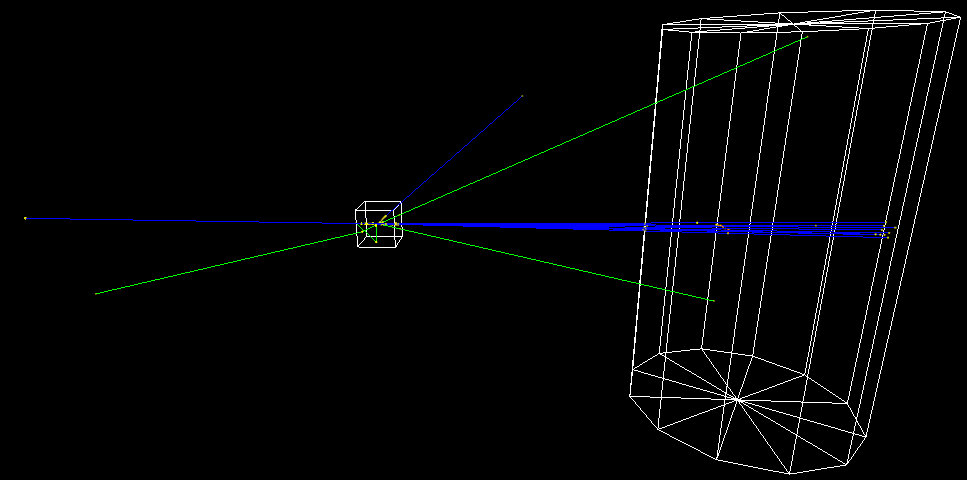
\includegraphics{pics/testrun.png}}
\caption{\small \emph{Schematic of constructed detector geometry with sample event, using Geant4 OpenGL visualization.}}
\label{fig:schematic}
\end{figurehere}
\vspace{0.25 cm}

The FTFP\_BERT 2.0 physics list was activated\cite{Geant4:physicsList}, with track cuts at a 10 micron minimum step legnth.  Primary particle energies range from $1$ to $5\cdot10^x$, where $x:\mathcal{Z}\in[0,8]$.

\subsection{Energy Deposition Tracking}

To acquire an energy deposition map of proton and neutron events in this physical setup, a script was introduced into the UserSteppingAction class.  This script acquired the position (in mm) and energy (in MeV) of every collision (G4Step) per event.  A UserRunAction method took averages ofenergy depositions throughout the 1150 mm world per bin, event, primary energy (G4Run) and geometry.

\subsection{Charge Deposition Tracking}

The charge deposition map for the proton and neutron events also utilized a UserSteppingAction script to obtain spatial values of charge displacement.  Dividing the world into (mm) bins, charge values of particles which gained momentum per event are subtracted from the bin of track vertex and added to the bin of track end.  The end of each G4Run included an averaging of the net charge per bin, event, energy and geometry; this net charge signature depicts the average polarization of the detectors.

\subsection{Particle Production Tracking}

Probably particle production matrices $P(n,m)$ were constructed by probing each G4Step which marked the end of a secondary particle's track for the particle name.  Gamma rays (indicitive of secondary electron production), as well as $n\times m$ combinations of secondary protons and neutrons for $n,m:\mathcal{Z}\in[1,5], \lq 5+$' were tallied per event.  Each G4Run ended by averaging the productions combinations by event per energy and geometry, normalizing the result such that $\sum_n \sum_m P(n,m) = 1$.

\section{Results}

\subsection{Energy Deposition}

Energy deposition signatures were acquired for protons and neutrons.  Figures \ref{fig:pEDep_Al5_eV} and \ref{fig:pEDep_Al5_keV} show a monotonically increaing function of energy deposition across the experimental distance $z$ for protons in the eV to keV range.  The MeV-range (fig~\ref{fig:pEDep_Al5_MeV}) uniquely depicts a peak around 50 MeV before sharply declining throughout the next order of magnitude.  The Aluminum cube volume, which exists in the range (57.5 cm $\pm$ $L_{Al}/2$) where $L_{Al}=5,10,25$ cm, receives virtually all protons until MeV-range energies.  Up to 20 MeV, the total energy is deposited at $z=57.5 cm - L_{Al}/2$, after which the total deposition extends further in the $+z$ direction.  The last decade of energy probed exibits a dramatic increase in this extension, which increasingly exposes a gradual incline to a peak followed by a drop.

%% Proton EDep figures
\vspace{0.15 cm}
\begin{figurehere}
\centering
\resizebox{\columnwidth}{!}{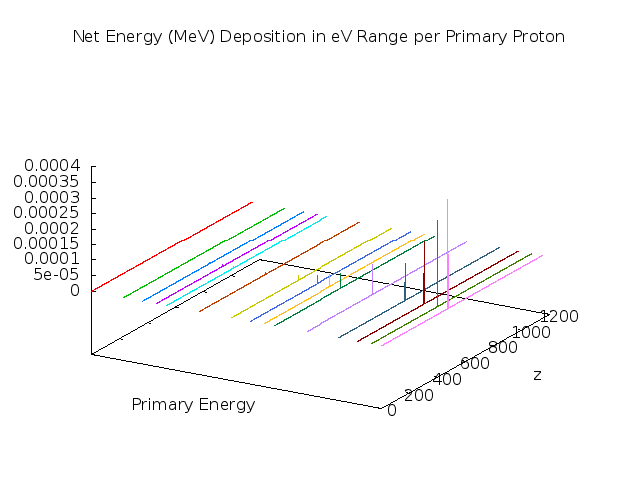
\includegraphics{pics/Al5/fig_pEDep_eV.png}}
\caption{\small \emph{Energy deposition landscape (MeV) per eV-range proton}}
\label{fig:pEDep_Al5_eV}
\end{figurehere}
\vspace{0.15 cm}
\begin{figurehere}
\centering
\resizebox{\columnwidth}{!}{\includegraphics{pics/Al5/fig_pEDep_keV.png}}
\caption{\small \emph{Energy deposition landscape (MeV) per keV-range proton}}
\label{fig:pEDep_Al5_keV}
\end{figurehere}
\vspace{0.15 cm}
\begin{figurehere}
\centering
\resizebox{\columnwidth}{!}{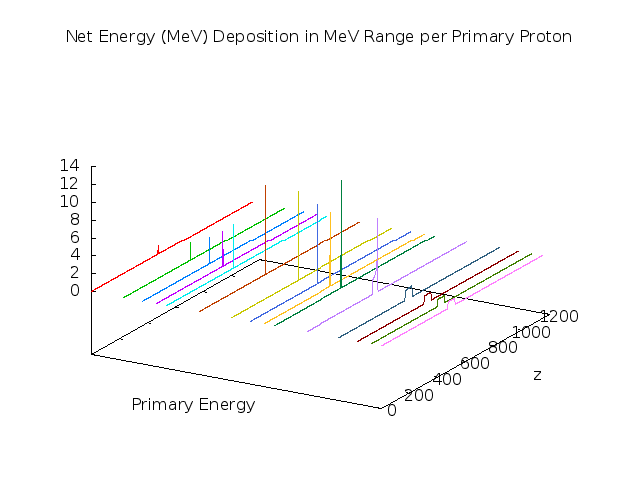
\includegraphics{pics/Al5/fig_pEDep_MeV.png}}
\caption{\small \emph{Energy deposition landscape (MeV) per MeV-range proton}}
\label{fig:pEDep_Al5_MeV}
\end{figurehere}
\vspace{0.15 cm}

%% Neutron EDep figures
\vspace{0.15 cm}
\begin{figurehere}
\centering
\resizebox{\columnwidth}{!}{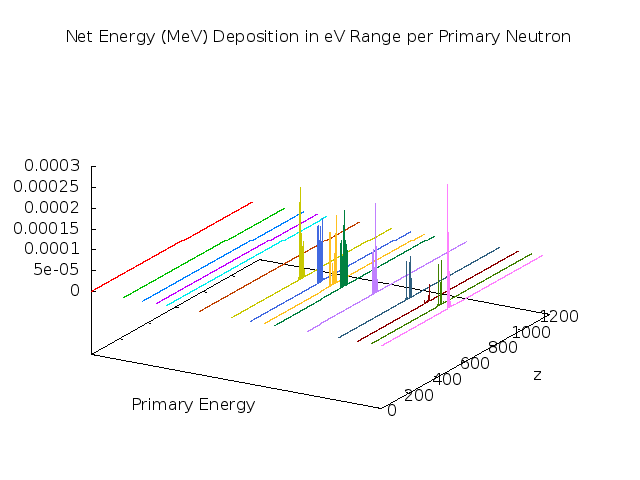
\includegraphics{pics/Al5/fig_nEDep_eV.png}}
\caption{\small \emph{Energy deposition landscape (MeV) per eV-range neutron}}
\label{fig:nEDep_Al5_eV}
\end{figurehere}
\vspace{0.15 cm}
\begin{figurehere}
\centering
\resizebox{\columnwidth}{!}{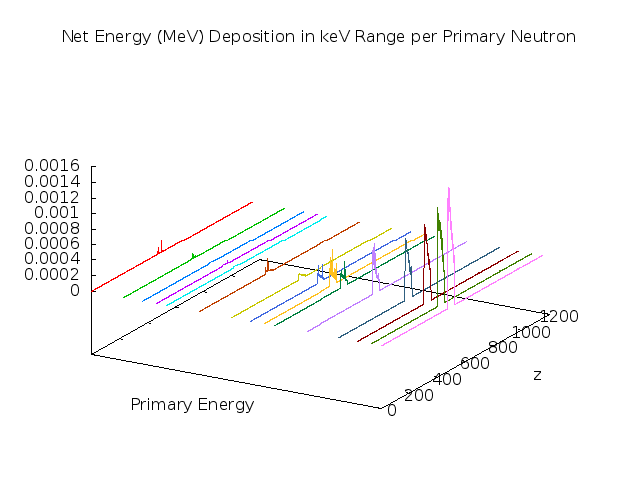
\includegraphics{pics/Al5/fig_nEDep_keV.png}}
\caption{\small \emph{Energy deposition landscape (MeV) per keV-range neutron}}
\label{fig:nEDep_Al5_keV}
\end{figurehere}
\vspace{0.15 cm}
\begin{figurehere}
\centering
\resizebox{\columnwidth}{!}{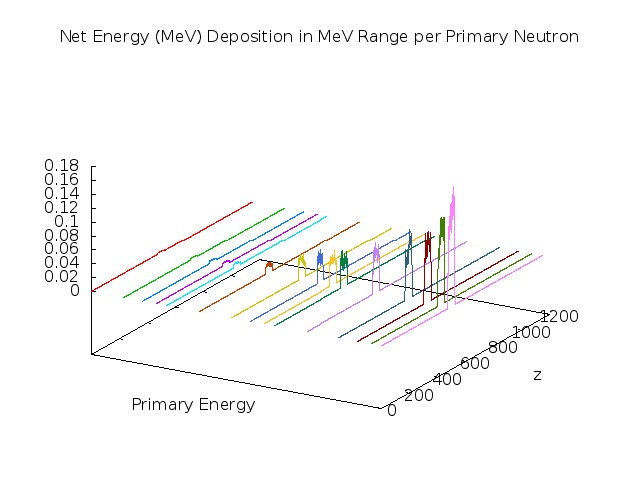
\includegraphics{pics/Al5/fig_nEDep_MeV.png}}
\caption{\small \emph{Energy deposition landscape (MeV) per MeV-range neutron}}
\label{fig:nEDep_Al5_MeV}
\end{figurehere}
\vspace{0.2 cm}

Neutron energy deposition maps are found in figures \ref{fig:nEDep_Al5_eV}, \ref{fig:nEDep_Al5_keV}, and \ref{fig:nEDep_Al5_MeV}, following the same energy labeling schema.  The total energy deposition here seems to monotonically increase indefinitely; upon reaching MeV-range energies, deposition distributes itself relatively evenly with a bias towards the right across the $57.5 cm \pm L_{Al}/2$ domain in $z$.  See Appendix~\ref{app:EDep} for energy deposition figures for secondary and tertiary geometric models, omitted for behavioral redundancy.


\subsection{Charge Deposition}

The average charge displacement per proton event is acquired and normalized by the gain equation (eqn.~\ref{eqn:gain}) in order to create a charge displacement landscapes.
\begin{equation}
  gain[z] = \frac{\sum \text{\emph{net charge @ z}} }{\sum \text{\emph{charge of primary particle}} } \label{eqn:gain}
\end{equation}
Up to around 10 keV proton energies (figs.~\ref{fig:pChargeDep_Al5_eV} and \ref{fig:pChargeDep_Al5_keV}) the nominal gain outside of the defined volumes (hence in air) are comparable to the magnitudes found between the boundaries of the Aluminum block.  Beyond 100 MeV proton energies (fig.~\ref{fig:pChargeDep_Al5_MeV}) a gain measurement may be found within the confines of the Helium cylinder, which exists within the range $z=100 cm \pm R_{He}$; for these figures, a large peak may be seen at the world's edge, $z=115 cm$.  The $-1e$ net gain at $z=0$ for all figures is where the collimated source originates.

No visible charge trasfer occurs with neutron primary events in the ev to keV energy range (figs.~\ref{fig:nChargeDep_Al5_eV} and \ref{fig:nChargeDep_Al5_keV}).  Only in MeV range beam energies (fig.~\ref{fig:nChargeDep_Al5_MeV}) do the neutron events charge transfer at the boundaries of both the Aluminum cube and Helium cylinder. See Appendix~\ref{app:ChargeDep} for charge deposition figures for secondary and tertiary geometric models, omitted for behavioral redundancy.


%% Proton ChargeDep figures
\vspace{0.15 cm}
\begin{figurehere}
\centering
\resizebox{\columnwidth}{!}{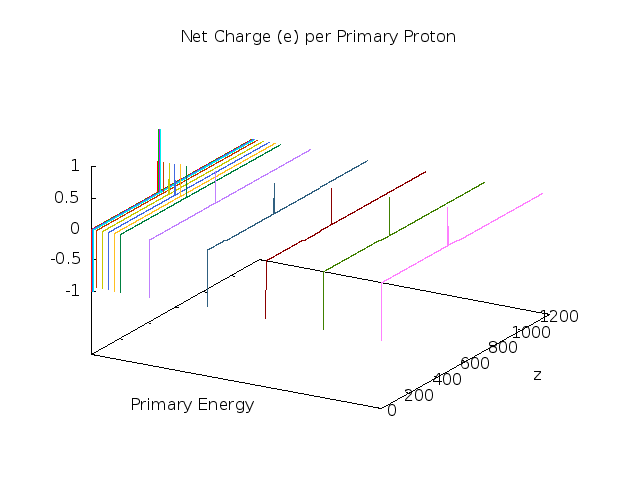
\includegraphics{pics/Al5/fig_pChargeDep_eV.png}}
\caption{\small \emph{Charge displacement landscape (gain) per eV-range proton}}
\label{fig:pChargeDep_Al5_eV}
\end{figurehere}
\vspace{0.15 cm}
\begin{figurehere}
\centering
\resizebox{\columnwidth}{!}{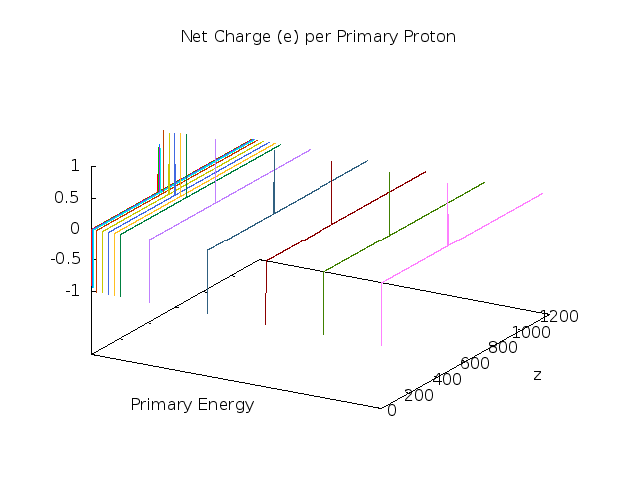
\includegraphics{pics/Al5/fig_pChargeDep_keV.png}}
\caption{\small \emph{Charge displacement landscape (gain) per keV-range proton}}
\label{fig:pChargeDep_Al5_keV}
\end{figurehere}
\vspace{0.15 cm}
\begin{figurehere}
\centering
\resizebox{\columnwidth}{!}{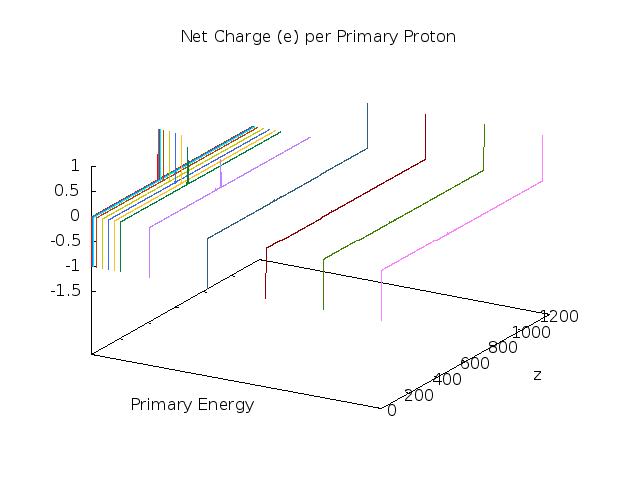
\includegraphics{pics/Al5/fig_pChargeDep_MeV.png}}
\caption{\small \emph{Charge displacement landscape (gain) per MeV-range proton}}
\label{fig:pChargeDep_Al5_MeV}
\end{figurehere}
\vspace{0.15 cm}

%% Neutron ChargeDep figures
\vspace{0.15 cm}
\begin{figurehere}
\centering
\resizebox{\columnwidth}{!}{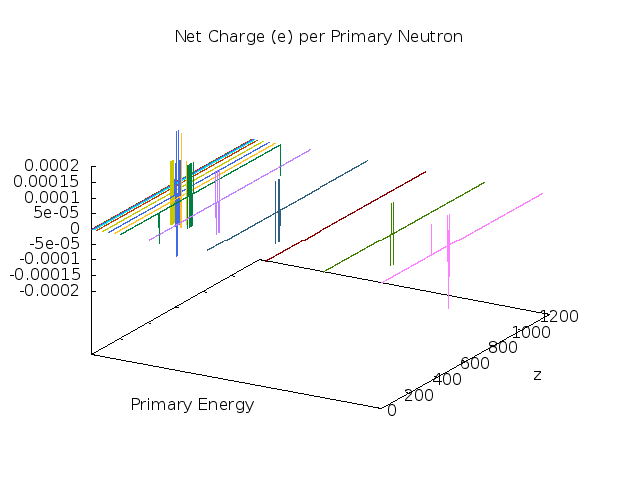
\includegraphics{pics/Al5/fig_nChargeDep_eV.png}}
\caption{\small \emph{Charge displacement landscape (gain) per eV-range neutron}}
\label{fig:nChargeDep_Al5_eV}
\end{figurehere}
\vspace{0.15 cm}
\begin{figurehere}
\centering
\resizebox{\columnwidth}{!}{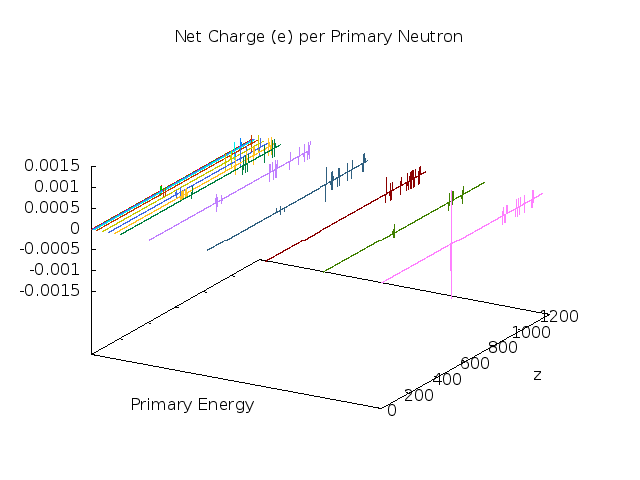
\includegraphics{pics/Al5/fig_nChargeDep_keV.png}}
\caption{\small \emph{Charge displacement landscape (gain) per keV-range neutron}}
\label{fig:nChargeDep_Al5_keV}
\end{figurehere}
\vspace{0.15 cm}
\begin{figurehere}
\centering
\resizebox{\columnwidth}{!}{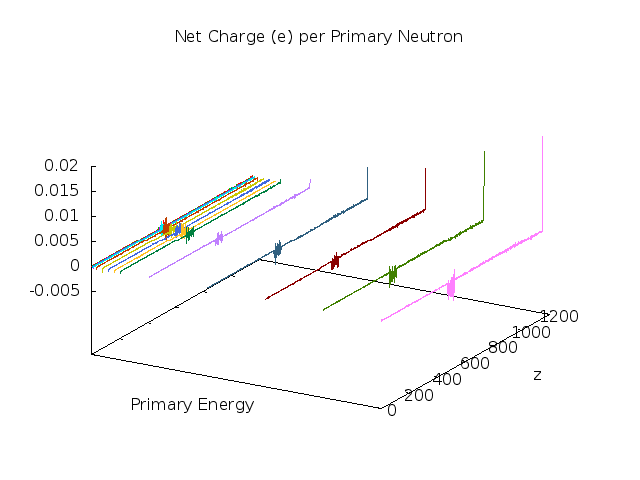
\includegraphics{pics/Al5/fig_nChargeDep_MeV.png}}
\caption{\small \emph{Charge displacement landscape (gain) per MeV-range neutron}}
\label{fig:nChargeDep_Al5_MeV}
\end{figurehere}
\vspace{0.15 cm}

\end{multicols}
\newpage
\subsection{Production Tallies}

There are no protons, neutrons nor gammas produced under 30 MeV proton beam energy, at which the number of gammas created per proton gradually increases with energy.  The first run which produced \emph{any} proton-neutron combination in any of the geometric setups occured at 200 MeV.  Particles production tallies for protons at 500 MeV are shown in tables \ref{tab:production_pAl5}, \ref{tab:production_pAl10}, and \ref{tab:production_pAl25}.

\vspace{0.15 cm}
\begin{tablehere}\begin{centering}
  \caption{\small \emph{Particle production combination probabilities per 500 MeV proton with $L_{Al}=5 cm$} (unnormalized)}
  \begin{tabular}{c || c c c c c c c}
    p vs. n & 0 & 1 & 2 & 3 & 4 & 5 & $>$5 \\
    \hline\hline
    0 & 1.0732 & 0.0043 & 0.0009 & 0.0004 & 0 & 0 & 0 \\
    1 & 0.204 & 0.0453 & 0.0117 & 0.0082 & 0.005 & 0.0003 & 0.0024 \\
    2 & 0.1664 & 0.0493 & 0.0482 & 0.0138 & 0.0055 & 0.0028 & 0.0055 \\
    3 & 0.0888 & 0.0227 & 0.0324 & 0.0159 & 0.0071 & 0.0044 & 0.003 \\
    4 & 0.0476 & 0.0212 & 0.0259 & 0.021 & 0.0193 & 0.0127 & 0.0076 \\
    5 & 0.0221 & 0.0079 & 0.0073 & 0.0092 & 0.011 & 0.0068 & 0.0105 \\
    $>$5 & 0.0141 & 0.0065 & 0.0067 & 0.0067 & 0.0092 & 0.0074 & 0.0195 \\
    \hline\hline
  \end{tabular} \\
  \begin{tabular}{r} Gammas: 1.0737 \end{tabular}
  \label{tab:production_pAl5}
\end{centering}\end{tablehere}
\vspace{0.15 cm}
\begin{tablehere}\begin{centering}
  \caption{\small \emph{Particle production combination probabilities per 500 MeV proton with $L_{Al}=10 cm$}}
  \begin{tabular}{c || c c c c c c c}
    p vs. n & 0 & 1 & 2 & 3 & 4 & 5 & $>$5 \\
    \hline\hline
    0 & 1.0494 & 0.0045 & 0.0015 & 0.0001 & 0.0001 & 0.0001 & 0.0004 \\
    1 & 0.225 & 0.0462 & 0.0115 & 0.0078 & 0.0044 & 0.0022 & 0.0001 \\
    2 & 0.1848 & 0.0576 & 0.0534 & 0.0183 & 0.0098 & 0.0027 & 0.0012 \\
    3 & 0.0942 & 0.0215 & 0.0309 & 0.0218 & 0.0075 & 0.0058 & 0.0035 \\
    4 & 0.0557 & 0.0192 & 0.0264 & 0.0198 & 0.0231 & 0.0124 & 0.0154 \\
    5 & 0.0238 & 0.0067 & 0.0068 & 0.0073 & 0.0095 & 0.0074 & 0.0071 \\
    $>$5 & 0.0173 & 0.0094 & 0.0089 & 0.0089 & 0.0086 & 0.0087 & 0.018 \\
    \hline\hline
  \end{tabular} \\
  \begin{tabular}{r} Gammas: 1.0871 \end{tabular}  
  \label{tab:production_pAl10}
\end{centering}\end{tablehere}
\vspace{0.15 cm}
\begin{tablehere}\begin{centering}
  \caption{\small \emph{Particle production combination probabilities per 500 MeV proton with $L_{Al}=25 cm$}}
  \begin{tabular}{c || c c c c c c c}
    p vs. n & 0 & 1 & 2 & 3 & 4 & 5 & $>$5 \\
    \hline\hline
    0 & 1.0647 & 0.004 & 0.0008 & 0.0001 & 0.0001 & 0.0001 & 0.0007 \\
    1 & 0.2215 & 0.0452 & 0.0086 & 0.0047 & 0.0014 & 0.0004 & 0.0006 \\
    2 & 0.1781 & 0.0554 & 0.056 & 0.0156 & 0.0059 & 0.0022 & 0.0035 \\
    3 & 0.1063 & 0.0232 & 0.0289 & 0.019 & 0.007 & 0.005 & 0.0046 \\
    4 & 0.0591 & 0.023 & 0.0265 & 0.0242 & 0.0217 & 0.0127 & 0.0111 \\
    5 & 0.0255 & 0.0077 & 0.0086 & 0.0093 & 0.0065 & 0.0048 & 0.0078 \\
    $>$5 & 0.0178 & 0.0098 & 0.0094 & 0.0103 & 0.0109 & 0.0134 & 0.0224 \\
    \hline\hline
  \end{tabular} \\
  \begin{tabular}{r} Gammas: 1.1055 \\ \end{tabular}  
  \label{tab:production_pAl25}
\end{centering}\end{tablehere}
\vspace{0.15 cm}

\begin{multicols}{2}
\section{Conclusions}

High energy protons were necessary to penetrate the Aluminum cube and consequentially bring visibility to the Bragg curve, characterized by the stopping power of protons in each media due to pathway ionization.  The total energy deposited into the volumes curiously seems to decrease beyond the peak with respect to beam energy in figure \ref{fig:pEDep_Al5_MeV}; what occurs here is a complete transmission of proportionately many protons through the Aluminum cube, and a continued travel of the protons into the Helium chamber, seen by the demonstrative schematic (fig.~\ref{fig:schematic}).  This phenomena reappears in the charge deposition landscape of protons at high energies (fig.~\ref{fig:pChargeDep_Al5_MeV}), where we observe a conspicuous gain at the world's edge, $z=115cm$; the protons must then tramsmit directly through the Helium chamber to the edge of the defined world where the fine $z$-bin collects the charge of the primary.

Neutrons, which do not ionize their penetration pathways, do not behave with a Bragg curve but rather undergo elastic scattering and nuclear interactions.  The resulting destructive recoil effect is shown by the development of a energy deposition bias in the Aluminum cube (figs.~\ref{fig:nEDep_Al5_eV}, \ref{fig:nEDep_Al5_keV}, \ref{fig:nEDep_Al5_MeV}).  Relatively few high energy neutrons are also found to transmit directly through the cube, evidenced by the small shifts in charge deposiition (fig.~\ref{fig:nChargeDep_Al5_MeV}) due to obliterated electrons travelling but tens of microns.

\begin{thebibliography}{99}

\bibitem[1]{Geant4:applications}
Geant4 Applications. \\
\url{http://geant4.web.cern.ch/geant4/applications/index.shtml}

\bibitem[2]{Geant4:physicsList}
\lq\lq Use cases - Reference Physics Lists." \\
Geant4 Online User Support. \\
\url{http://www.geant4.org/geant4/support/proc_mod_catalog/physics_lists/useCases.shtml}
 
\end{thebibliography}
\end{multicols}
\appendix
\newpage
\section{Energy deposition for Al side of 10, 25 cm}\label{app:EDep}

\begin{multicols}{2}

%% Proton EDep figures
\begin{figurehere}
\centering
\resizebox{0.9\columnwidth}{!}{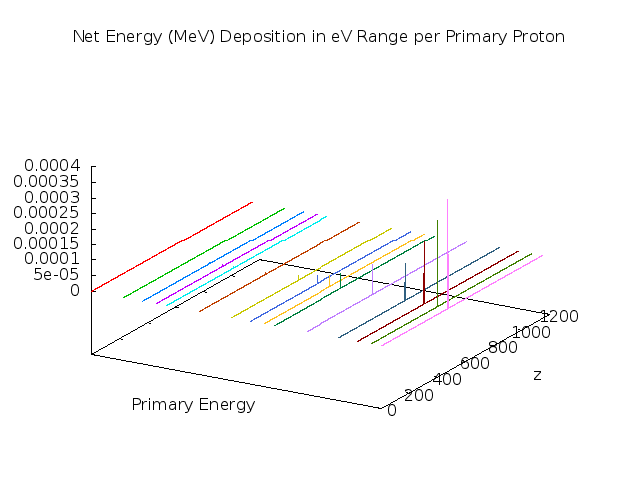
\includegraphics{pics/Al10/fig_pEDep_eV.png}}
\caption{\small \emph{Energy deposition landscape (MeV) per eV-range proton}}
\label{fig:pEDep_Al10_eV}
\end{figurehere}
\begin{figurehere}
\centering
\resizebox{0.9\columnwidth}{!}{\includegraphics{pics/Al10/fig_pEDep_keV.png}}
\caption{\small \emph{Energy deposition landscape (MeV) per keV-range proton}}
\label{fig:pEDep_Al10_keV}
\end{figurehere}
\begin{figurehere}
\centering
\resizebox{0.9\columnwidth}{!}{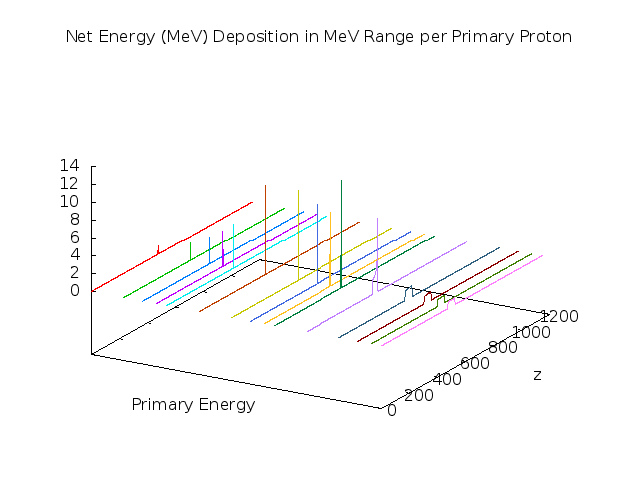
\includegraphics{pics/Al10/fig_pEDep_MeV.png}}
\caption{\small \emph{Energy deposition landscape (MeV) per MeV-range proton}}
\label{fig:pEDep_Al10_MeV}
\end{figurehere}

%% Neutron EDep figures
\begin{figurehere}
\centering
\resizebox{0.9\columnwidth}{!}{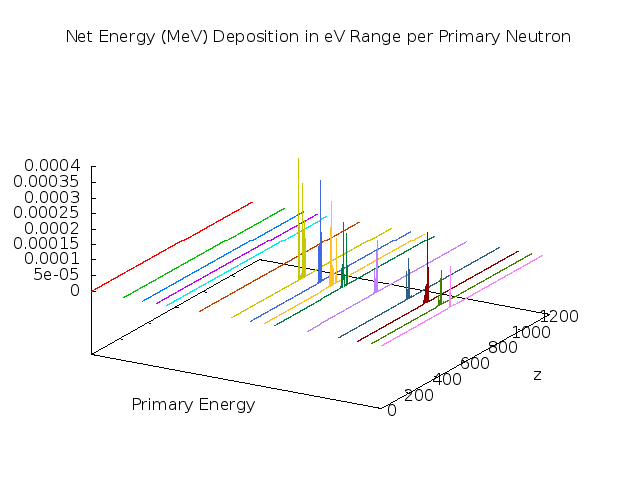
\includegraphics{pics/Al10/fig_nEDep_eV.png}}
\caption{\small \emph{Energy deposition landscape (MeV) per eV-range neutron}}
\label{fig:nEDep_Al10_eV}
\end{figurehere}
\begin{figurehere}
\centering
\resizebox{0.9\columnwidth}{!}{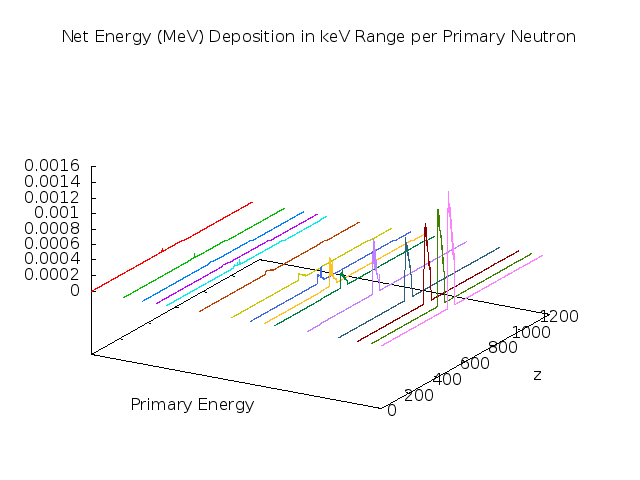
\includegraphics{pics/Al10/fig_nEDep_keV.png}}
\caption{\small \emph{Energy deposition landscape (MeV) per keV-range neutron}}
\label{fig:nEDep_Al10_keV}
\end{figurehere}
\begin{figurehere}
\centering
\resizebox{0.9\columnwidth}{!}{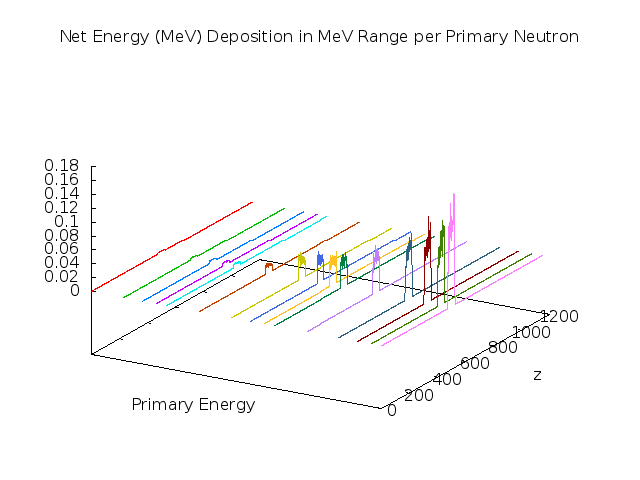
\includegraphics{pics/Al10/fig_nEDep_MeV.png}}
\caption{\small \emph{Energy deposition landscape (MeV) per MeV-range neutron}}
\label{fig:nEDep_Al10_MeV}
\end{figurehere}

%% Proton EDep figures
\vspace{0.15 cm}
\begin{figurehere}
\centering
\resizebox{\columnwidth}{!}{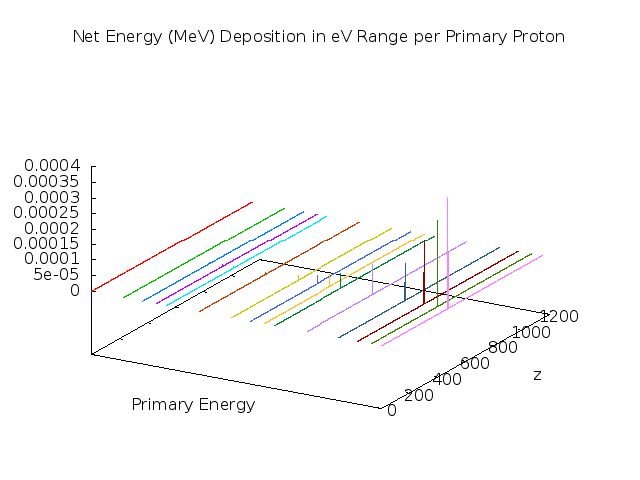
\includegraphics{pics/Al25/fig_pEDep_eV.png}}
\caption{\small \emph{Energy deposition landscape (MeV) per eV-range proton}}
\label{fig:pEDep_Al25_eV}
\end{figurehere}
\vspace{0.15 cm}
\begin{figurehere}
\centering
\resizebox{\columnwidth}{!}{\includegraphics{pics/Al25/fig_pEDep_keV.png}}
\caption{\small \emph{Energy deposition landscape (MeV) per keV-range proton}}
\label{fig:pEDep_Al25_keV}
\end{figurehere}
\vspace{0.15 cm}
\begin{figurehere}
\centering
\resizebox{\columnwidth}{!}{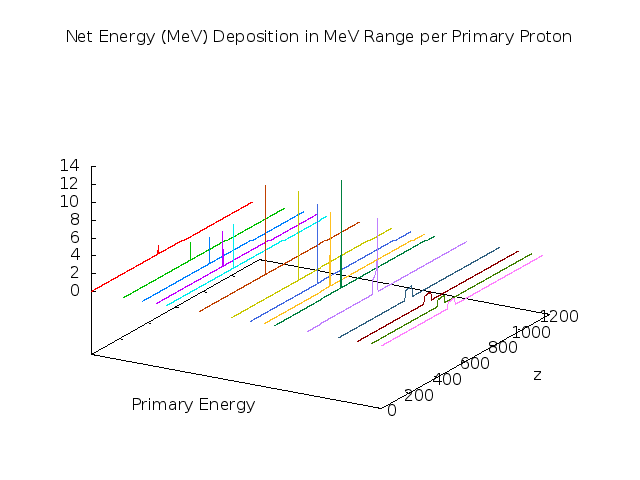
\includegraphics{pics/Al25/fig_pEDep_MeV.png}}
\caption{\small \emph{Energy deposition landscape (MeV) per MeV-range proton}}
\label{fig:pEDep_Al25_MeV}
\end{figurehere}
\vspace{0.15 cm}

%% Neutron EDep figures
\vspace{0.15 cm}
\begin{figurehere}
\centering
\resizebox{\columnwidth}{!}{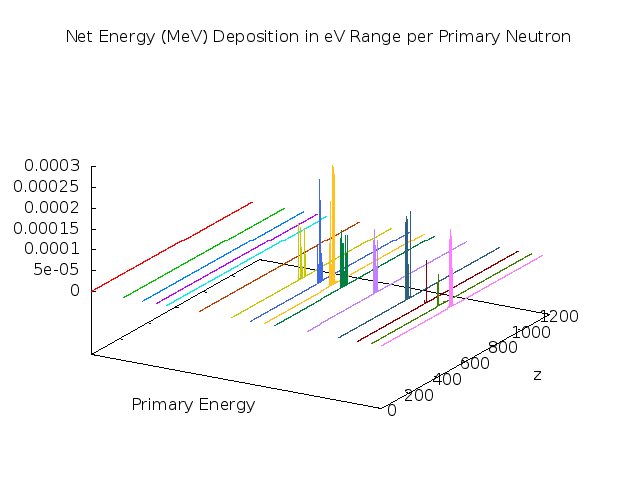
\includegraphics{pics/Al25/fig_nEDep_eV.png}}
\caption{\small \emph{Energy deposition landscape (MeV) per eV-range neutron}}
\label{fig:nEDep_Al25_eV}
\end{figurehere}
\vspace{0.15 cm}
\begin{figurehere}
\centering
\resizebox{\columnwidth}{!}{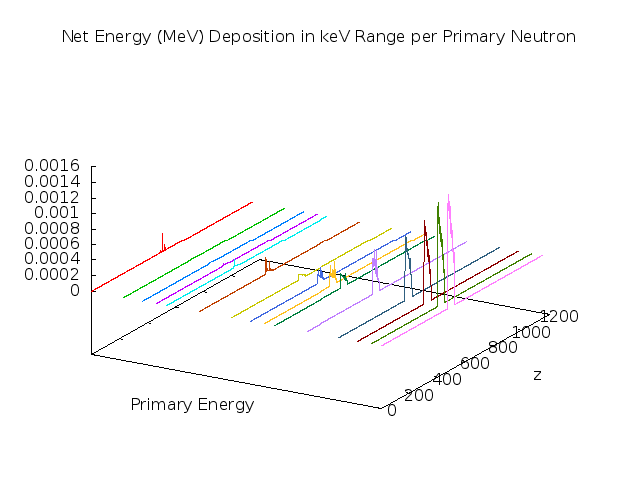
\includegraphics{pics/Al25/fig_nEDep_keV.png}}
\caption{\small \emph{Energy deposition landscape (MeV) per keV-range neutron}}
\label{fig:nEDep_Al25_keV}
\end{figurehere}
\vspace{0.15 cm}
\begin{figurehere}
\centering
\resizebox{\columnwidth}{!}{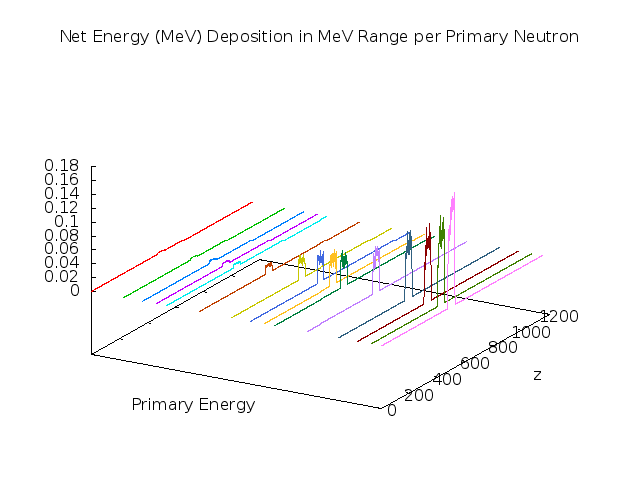
\includegraphics{pics/Al25/fig_nEDep_MeV.png}}
\caption{\small \emph{Energy deposition landscape (MeV) per MeV-range neutron}}
\label{fig:nEDep_Al25_MeV}
\end{figurehere}
\vspace{0.2 cm}

\end{multicols}
\newpage
\section{Charge deposition for Al side of 10, 25 cm}\label{app:ChargeDep}

\begin{multicols}{2}

%% Proton ChargeDep figures
\vspace{0.15 cm}
\begin{figurehere}
\centering
\resizebox{0.9\columnwidth}{!}{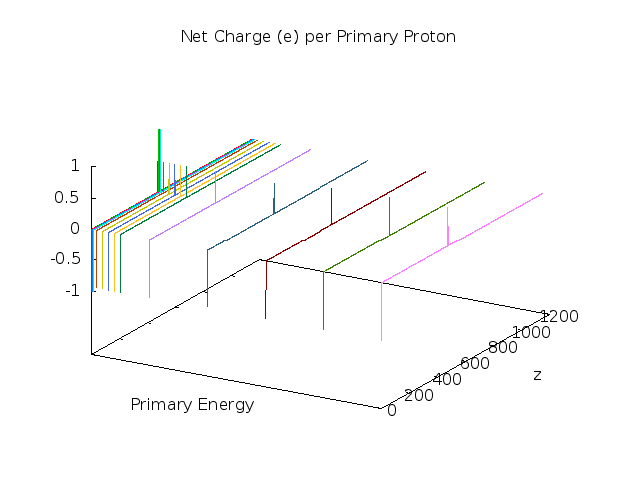
\includegraphics{pics/Al10/fig_pChargeDep_eV.png}}
\caption{\small \emph{Charge displacement landscape (gain) per eV-range proton}}
\label{fig:pChargeDep_Al10_eV}
\end{figurehere}
\vspace{0.15 cm}
\begin{figurehere}
\centering
\resizebox{0.9\columnwidth}{!}{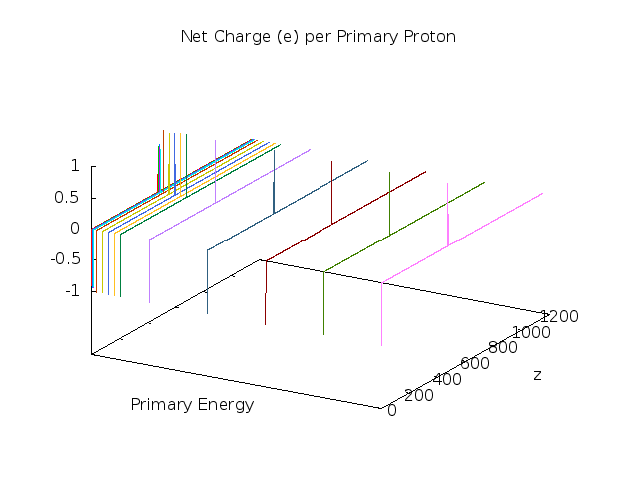
\includegraphics{pics/Al10/fig_pChargeDep_keV.png}}
\caption{\small \emph{Charge displacement landscape (gain) per keV-range proton}}
\label{fig:pChargeDep_Al10_keV}
\end{figurehere}
\vspace{0.15 cm}
\begin{figurehere}
\centering
\resizebox{0.9\columnwidth}{!}{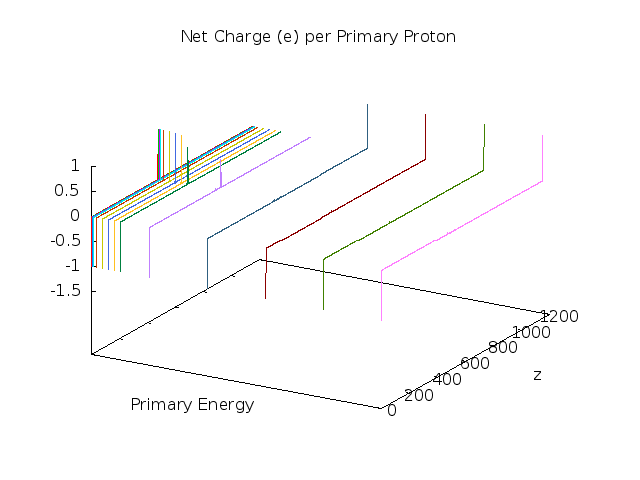
\includegraphics{pics/Al10/fig_pChargeDep_MeV.png}}
\caption{\small \emph{Charge displacement landscape (gain) per MeV-range proton}}
\label{fig:pChargeDep_Al10_MeV}
\end{figurehere}
\vspace{0.15 cm}

%% Neutron ChargeDep figures
\vspace{0.15 cm}
\begin{figurehere}
\centering
\resizebox{0.9\columnwidth}{!}{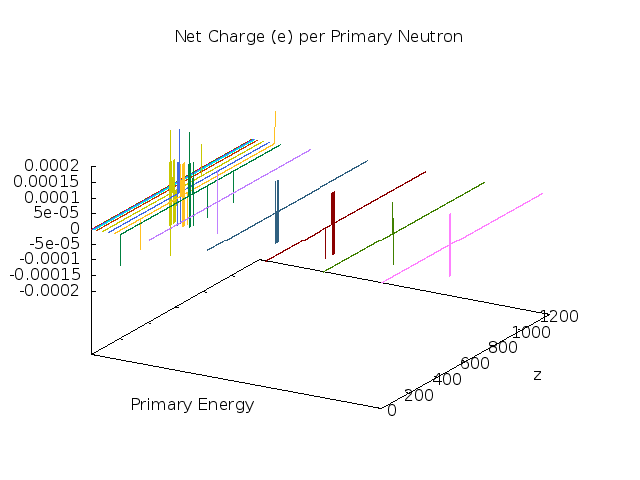
\includegraphics{pics/Al10/fig_nChargeDep_eV.png}}
\caption{\small \emph{Charge displacement landscape (gain) per eV-range neutron}}
\label{fig:nChargeDep_Al10_eV}
\end{figurehere}
\vspace{0.15 cm}
\begin{figurehere}
\centering
\resizebox{0.9\columnwidth}{!}{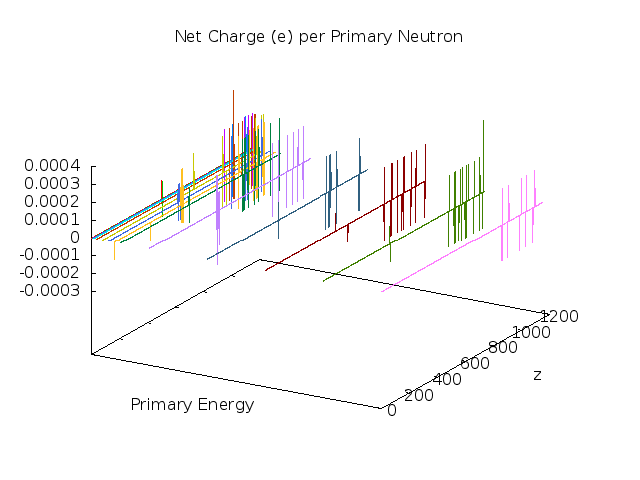
\includegraphics{pics/Al10/fig_nChargeDep_keV.png}}
\caption{\small \emph{Charge displacement landscape (gain) per keV-range neutron}}
\label{fig:nChargeDep_Al10_keV}
\end{figurehere}
\vspace{0.15 cm}
\begin{figurehere}
\centering
\resizebox{0.9\columnwidth}{!}{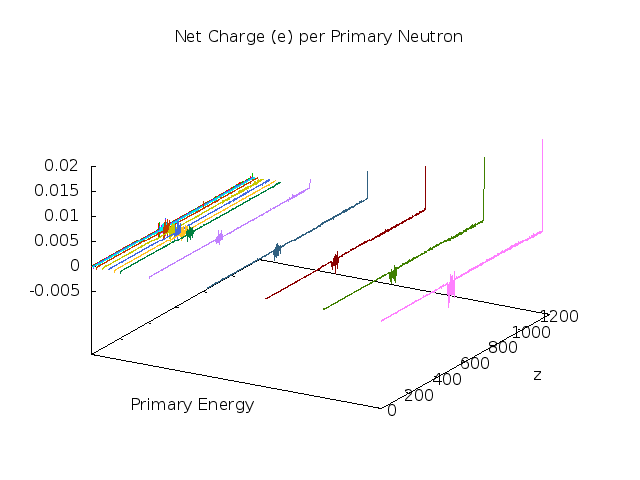
\includegraphics{pics/Al10/fig_nChargeDep_MeV.png}}
\caption{\small \emph{Charge displacement landscape (gain) per MeV-range neutron}}
\label{fig:nChargeDep_Al10_MeV}
\end{figurehere}
\vspace{0.15 cm}

%% Proton ChargeDep figures
\vspace{0.15 cm}
\begin{figurehere}
\centering
\resizebox{\columnwidth}{!}{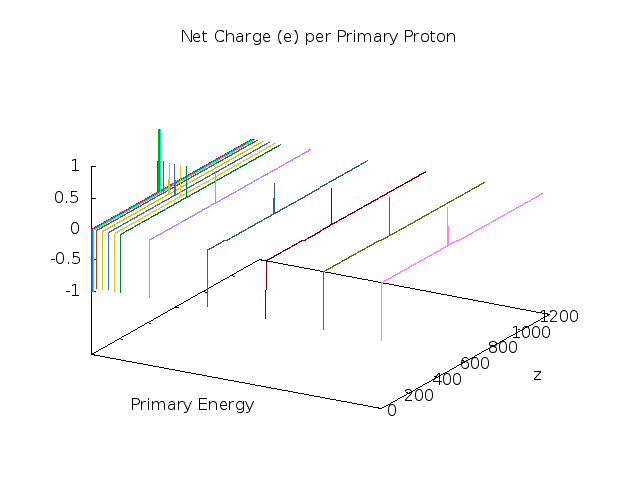
\includegraphics{pics/Al25/fig_pChargeDep_eV.png}}
\caption{\small \emph{Charge displacement landscape (gain) per eV-range proton}}
\label{fig:pChargeDep_Al25_eV}
\end{figurehere}
\vspace{0.15 cm}
\begin{figurehere}
\centering
\resizebox{\columnwidth}{!}{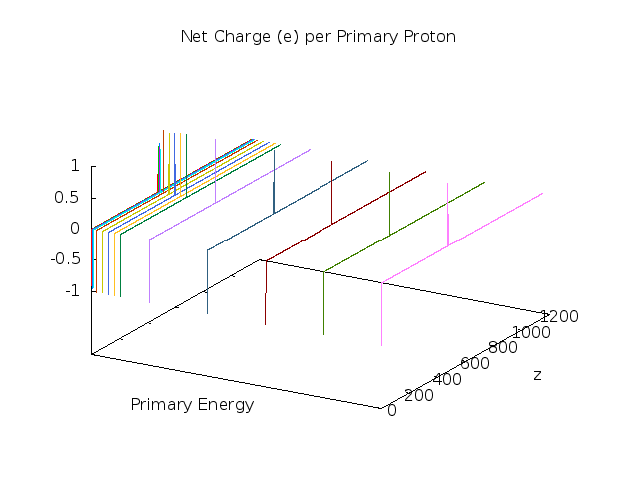
\includegraphics{pics/Al25/fig_pChargeDep_keV.png}}
\caption{\small \emph{Charge displacement landscape (gain) per keV-range proton}}
\label{fig:pChargeDep_Al25_keV}
\end{figurehere}
\vspace{0.15 cm}
\begin{figurehere}
\centering
\resizebox{\columnwidth}{!}{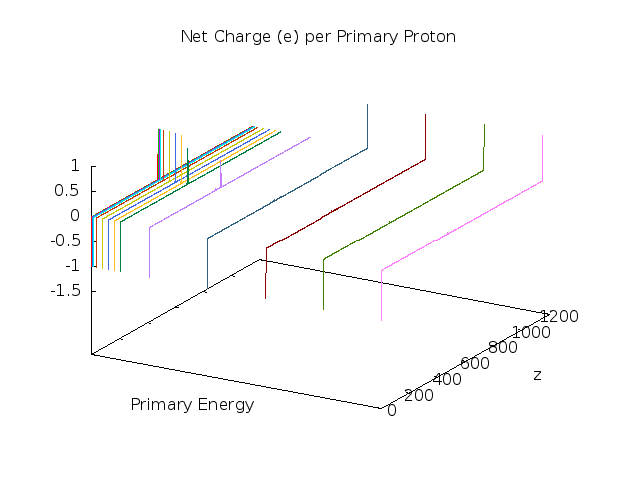
\includegraphics{pics/Al25/fig_pChargeDep_MeV.png}}
\caption{\small \emph{Charge displacement landscape (gain) per MeV-range proton}}
\label{fig:pChargeDep_Al25_MeV}
\end{figurehere}
\vspace{0.15 cm}

%% Neutron ChargeDep figures
\vspace{0.15 cm}
\begin{figurehere}
\centering
\resizebox{\columnwidth}{!}{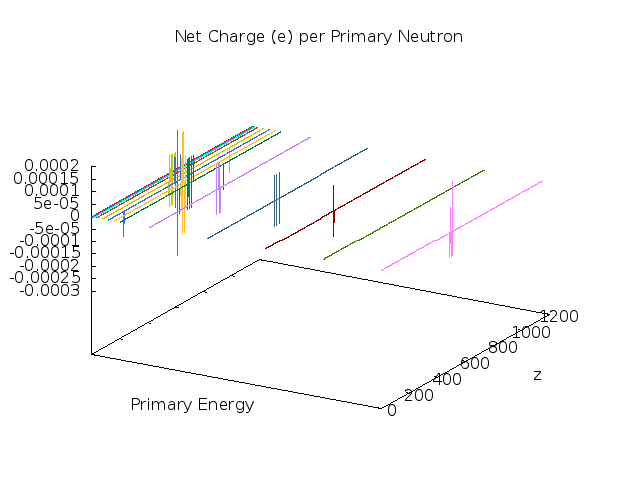
\includegraphics{pics/Al25/fig_nChargeDep_eV.png}}
\caption{\small \emph{Charge displacement landscape (gain) per eV-range neutron}}
\label{fig:nChargeDep_Al25_eV}
\end{figurehere}
\vspace{0.15 cm}
\begin{figurehere}
\centering
\resizebox{\columnwidth}{!}{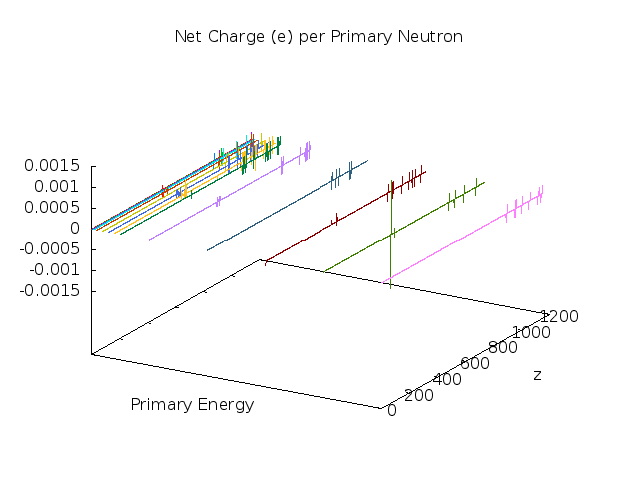
\includegraphics{pics/Al25/fig_nChargeDep_keV.png}}
\caption{\small \emph{Charge displacement landscape (gain) per keV-range neutron}}
\label{fig:nChargeDep_Al25_keV}
\end{figurehere}
\vspace{0.15 cm}
\begin{figurehere}
\centering
\resizebox{\columnwidth}{!}{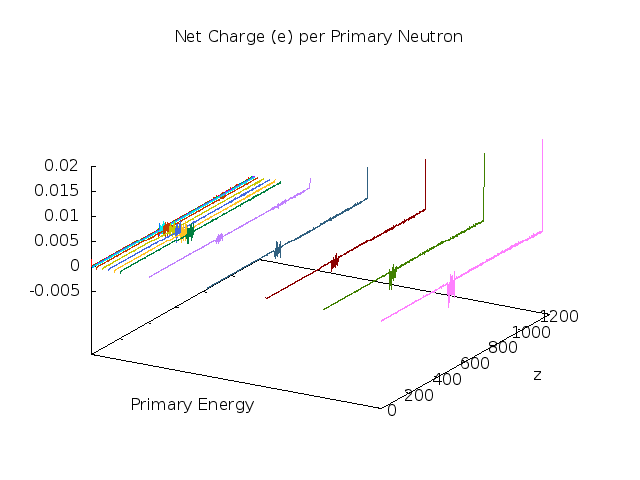
\includegraphics{pics/Al25/fig_nChargeDep_MeV.png}}
\caption{\small \emph{Charge displacement landscape (gain) per MeV-range neutron}}
\label{fig:nChargeDep_Al25_MeV}
\end{figurehere}
\vspace{0.15 cm}

\end{multicols}
\end{document}
